\documentclass[UTF8,AutoFakeBold,a4paper]{article}  %支持粗体
\usepackage{ctex}   % 支持中文编码
\usepackage[top=1in,bottom=1in,right=3.18cm,left=3.18cm]{geometry}   % 页边距调整
\usepackage{graphicx}   % 图片支持
\usepackage{float}      % 图片强制放置
\usepackage{indentfirst}% 首行缩进
\usepackage{titlesec}   % 设置标题
\usepackage{zhnumber}   % 设置中文section序号
\usepackage{amsmath,amssymb}    % 数学公式
\usepackage{enumerate, enumitem}    % 设置序号单元
\usepackage[thinlines]{easytable}   % 创建简单表格

% 设置中文section序号
\titleformat{\section}[block]{\zihao{4}\bfseries\fangsong}{\zhnum{section}、}{0em}{}[]
% 首行缩进
\setlength{\parindent}{2em}
% 图片下方注释
\newenvironment{fignote}{\begin{quote}\footnotesize}{\end{quote}}

\begin{document}
    \thispagestyle{empty}
    \begin{figure}[t]
        \centering
        
\includegraphics[width=4.3cm]{figures/zju_subnote.png}
        \textbf{\zihao{1}\bfseries\kaishu 实验报告}
    \end{figure}
    \parbox{0.9\linewidth}{
        \fangsong\zihao{4}\linespread{1.5}
        课程名称:\underline{\hbox to 0.33\linewidth{\hfill 流体力学 \hfill}}
        实验类型:\underline{\hbox to 0.32\linewidth{\hfill 验证性 \hfill}} \\ 
        实验项目名称:\underline{\hbox to 0.75\linewidth{\hfill \hfill}} \\ 
        学生姓名:\underline{\hbox to 0.2\linewidth{\hfill \hfill}}
        专业:\underline{\hbox to 0.2\linewidth{\hfill \hfill}}
        学号:\underline{\hbox to 0.2\linewidth{\hfill \hfill}} \\ 
        同组学生姓名:	\underline{\hbox to 0.75\linewidth{\hfill \hfill}} \\ 		         		
        指导老师:\underline{\hbox to 0.83\linewidth{\hfill \hfill}} \\ 
        实验地点:\underline{\hbox to 0.31\linewidth{\hfill \hfill}}
        实验日期:\underline{\hbox to 0.05\linewidth{\hfill \hfill}}年
        \underline{\hbox to 0.05\linewidth{\hfill \hfill}}月
        \underline{\hbox to 0.05\linewidth{\hfill \hfill}}日
    }
    \section{实验目的和要求}
    \section{实验内容和原理}
    \section{主要仪器设备}
    \begin{figure}[H]
        \centering 
        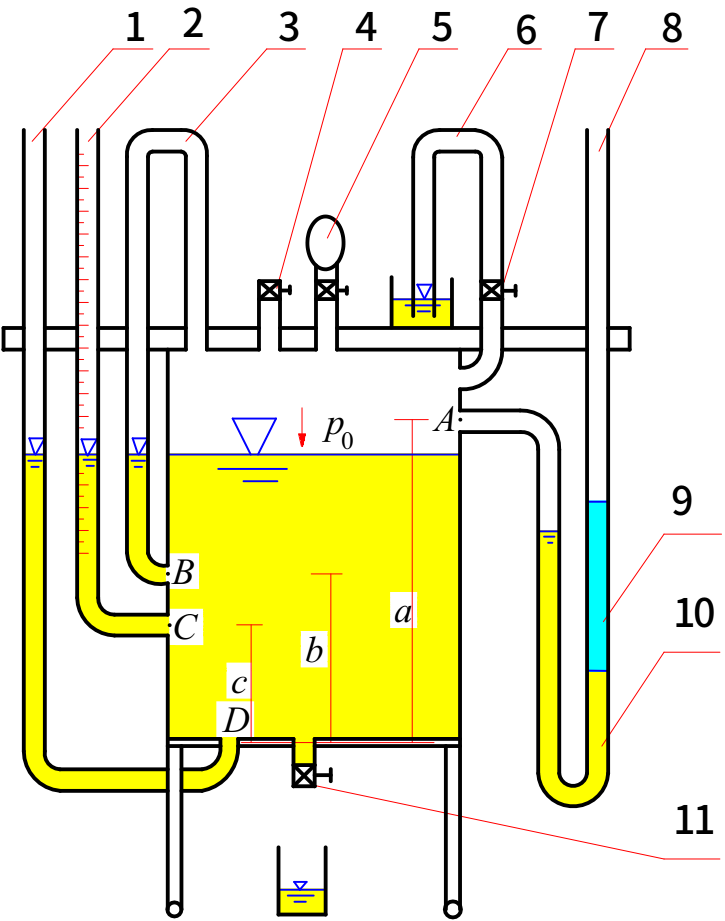
\includegraphics[width=0.4\linewidth]{figures/exp1.png}
        \caption{\zihao{5}流体静力学综合型实验装置图}
        \par
        {\zihao{5}\noindent 1. 测压管 \quad 2. 带标尺测压管 \quad 3. 连通管 \quad 4. 通气阀 \quad 5. 加压打气球 \\ 
        6. 真空测压管 \quad 7. 截止阀 \quad 8. U型测压管 \quad 9. 油柱 \quad 10. 水柱 \quad 11. 减压放水阀 \par}
    \end{figure}        
    \section{操作方法与实验步骤}
    \section{实验数据记录和处理}
    \begin{enumerate}
        \linespread{1.5}
        \item 记录有关信息及实验常数
        \par 
        实验设备名称:\underline{\hbox to 0.4\linewidth{\hfill \hfill}}
        实验台号:\underline{\hbox to 0.2\linewidth{\hfill \hfill}} \\ 
        实验者:\underline{\hbox to 0.48\linewidth{\hfill \hfill}}
        实验日期:\underline{\hbox to 0.2\linewidth{\hfill \hfill}} \\ 
        各测点高程为:
        $ \nabla_{B}= $\underline{\hbox to 0.1\linewidth{\hfill \hfill}}$ \times10^{-2}\mathrm{m} $,
        $ \nabla_{C}= $\underline{\hbox to 0.1\linewidth{\hfill \hfill}}$ \times10^{-2}\mathrm{m} $,
        $ \nabla_{D}= $\underline{\hbox to 0.1\linewidth{\hfill \hfill}}$ \times10^{-2}\mathrm{m} $ \\ 
        基准面选在\underline{\hbox to 0.33\linewidth{\hfill \hfill}},
        $ z_{C}= $\underline{\hbox to 0.1\linewidth{\hfill \hfill}}$ \times10^{-2}\mathrm{m} $
        $ z_{D}= $\underline{\hbox to 0.1\linewidth{\hfill \hfill}}$ \times10^{-2}\mathrm{m} $
        \item 实验数据记录及计算结果(参表1,表2)
    \end{enumerate}
    \section{实验结果与分析}
    \section{分析思考}
\end{document}